\documentclass[]{article}  % Comment this line out

%\IEEEoverridecommandlockouts                              % This command is only
                                                          % needed if you want to
                                                          % use the \thanks command
%\overrideIEEEmargins

\usepackage[margin=1in]{geometry}
\usepackage{amsmath}    % need for subequations
\usepackage{graphicx}   % need for figures
\usepackage[font=footnotesize,labelfont=footnotesize]{caption}
\usepackage{verbatim}   % useful for program listings
\usepackage{color}      % use if color is used in text
%\usepackage{begin{subfigure} % use for side-by-side figures
\usepackage{subcaption}
\usepackage{hyperref} % use for hypertext links, including those to external documents and URLs
\usepackage{multirow}
\usepackage{rotating}
\usepackage{array}
\usepackage{xspace}
\usepackage{indentfirst}
\usepackage{amssymb}
\usepackage{float}
\usepackage{algorithm}
\usepackage{algorithmic}
\usepackage{comment}
\usepackage{sidecap}
\usepackage{booktabs}

\newtheorem{theorem}{\bf Theorem}
\newtheorem{todo}{\bf Todo}
\newtheorem{remark}{\bf Remark}
\newtheorem{corollary}{\bf Corollary}
\newtheorem{definition}{\bf Definition}
\newtheorem{lemma}{\bf Lemma}
\newtheorem{proposition}[theorem]{\bf Proposition}

\title{Analysis of Perturbations on Bounce Visibility}

\author{Alexandra Q. Nilles% <-this % stops a space
%\thanks{This work was partially supported by National Science Foundation (award numbers CMMI-1100579 and IIS-1302393).}
}

\begin{document}


\begin{figure}
\centering
\begin{subfigure}{0.33\textwidth}
  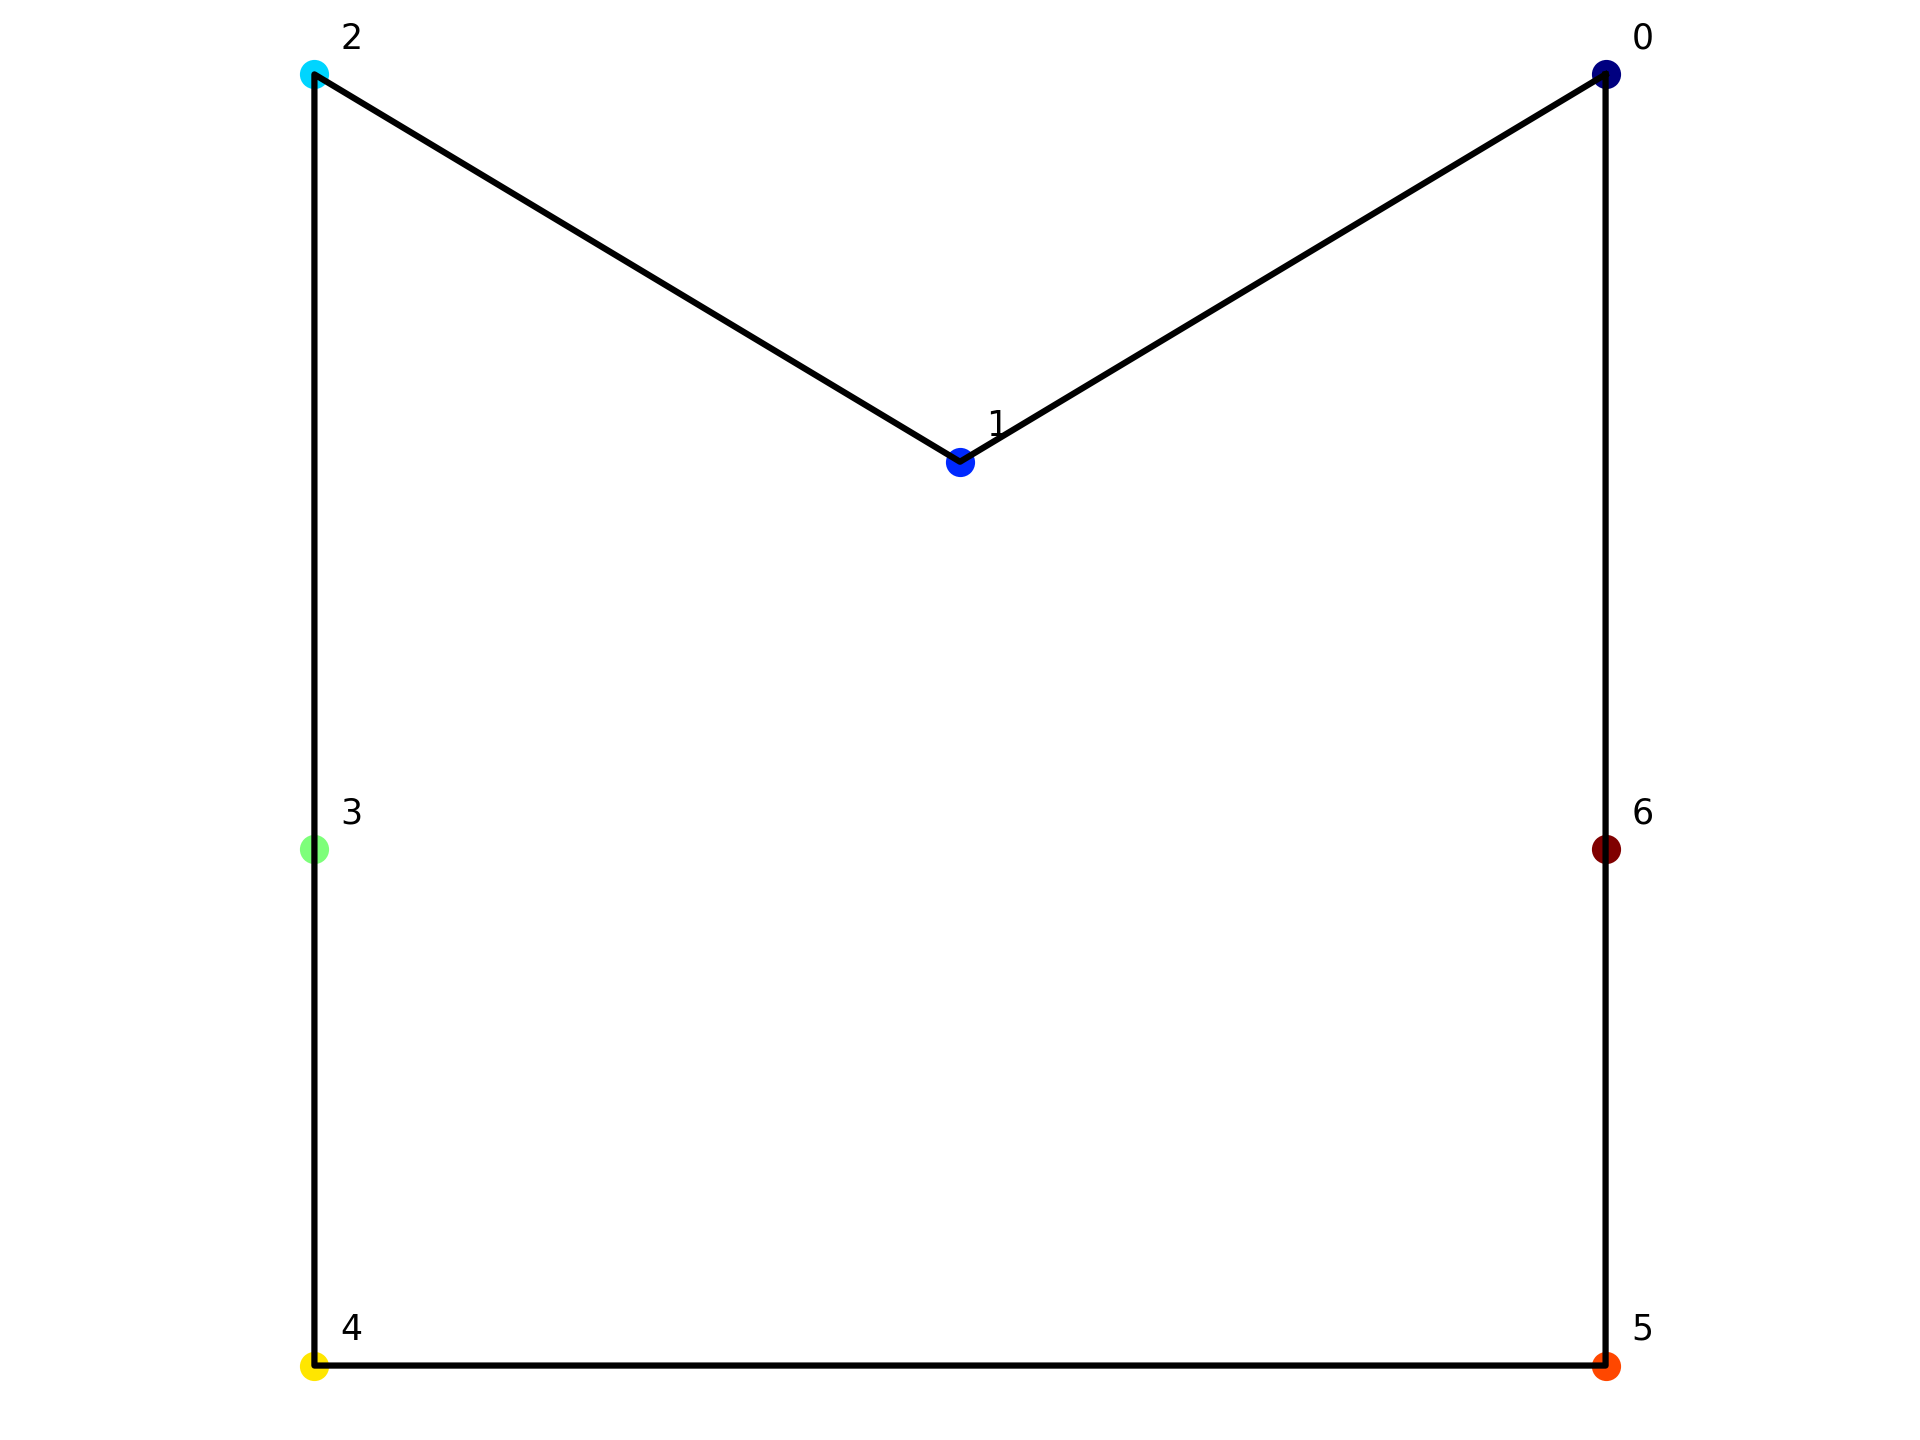
\includegraphics[width=\textwidth]{figures/poly1.png}
\end{subfigure}%
\begin{subfigure}{0.33\textwidth}
  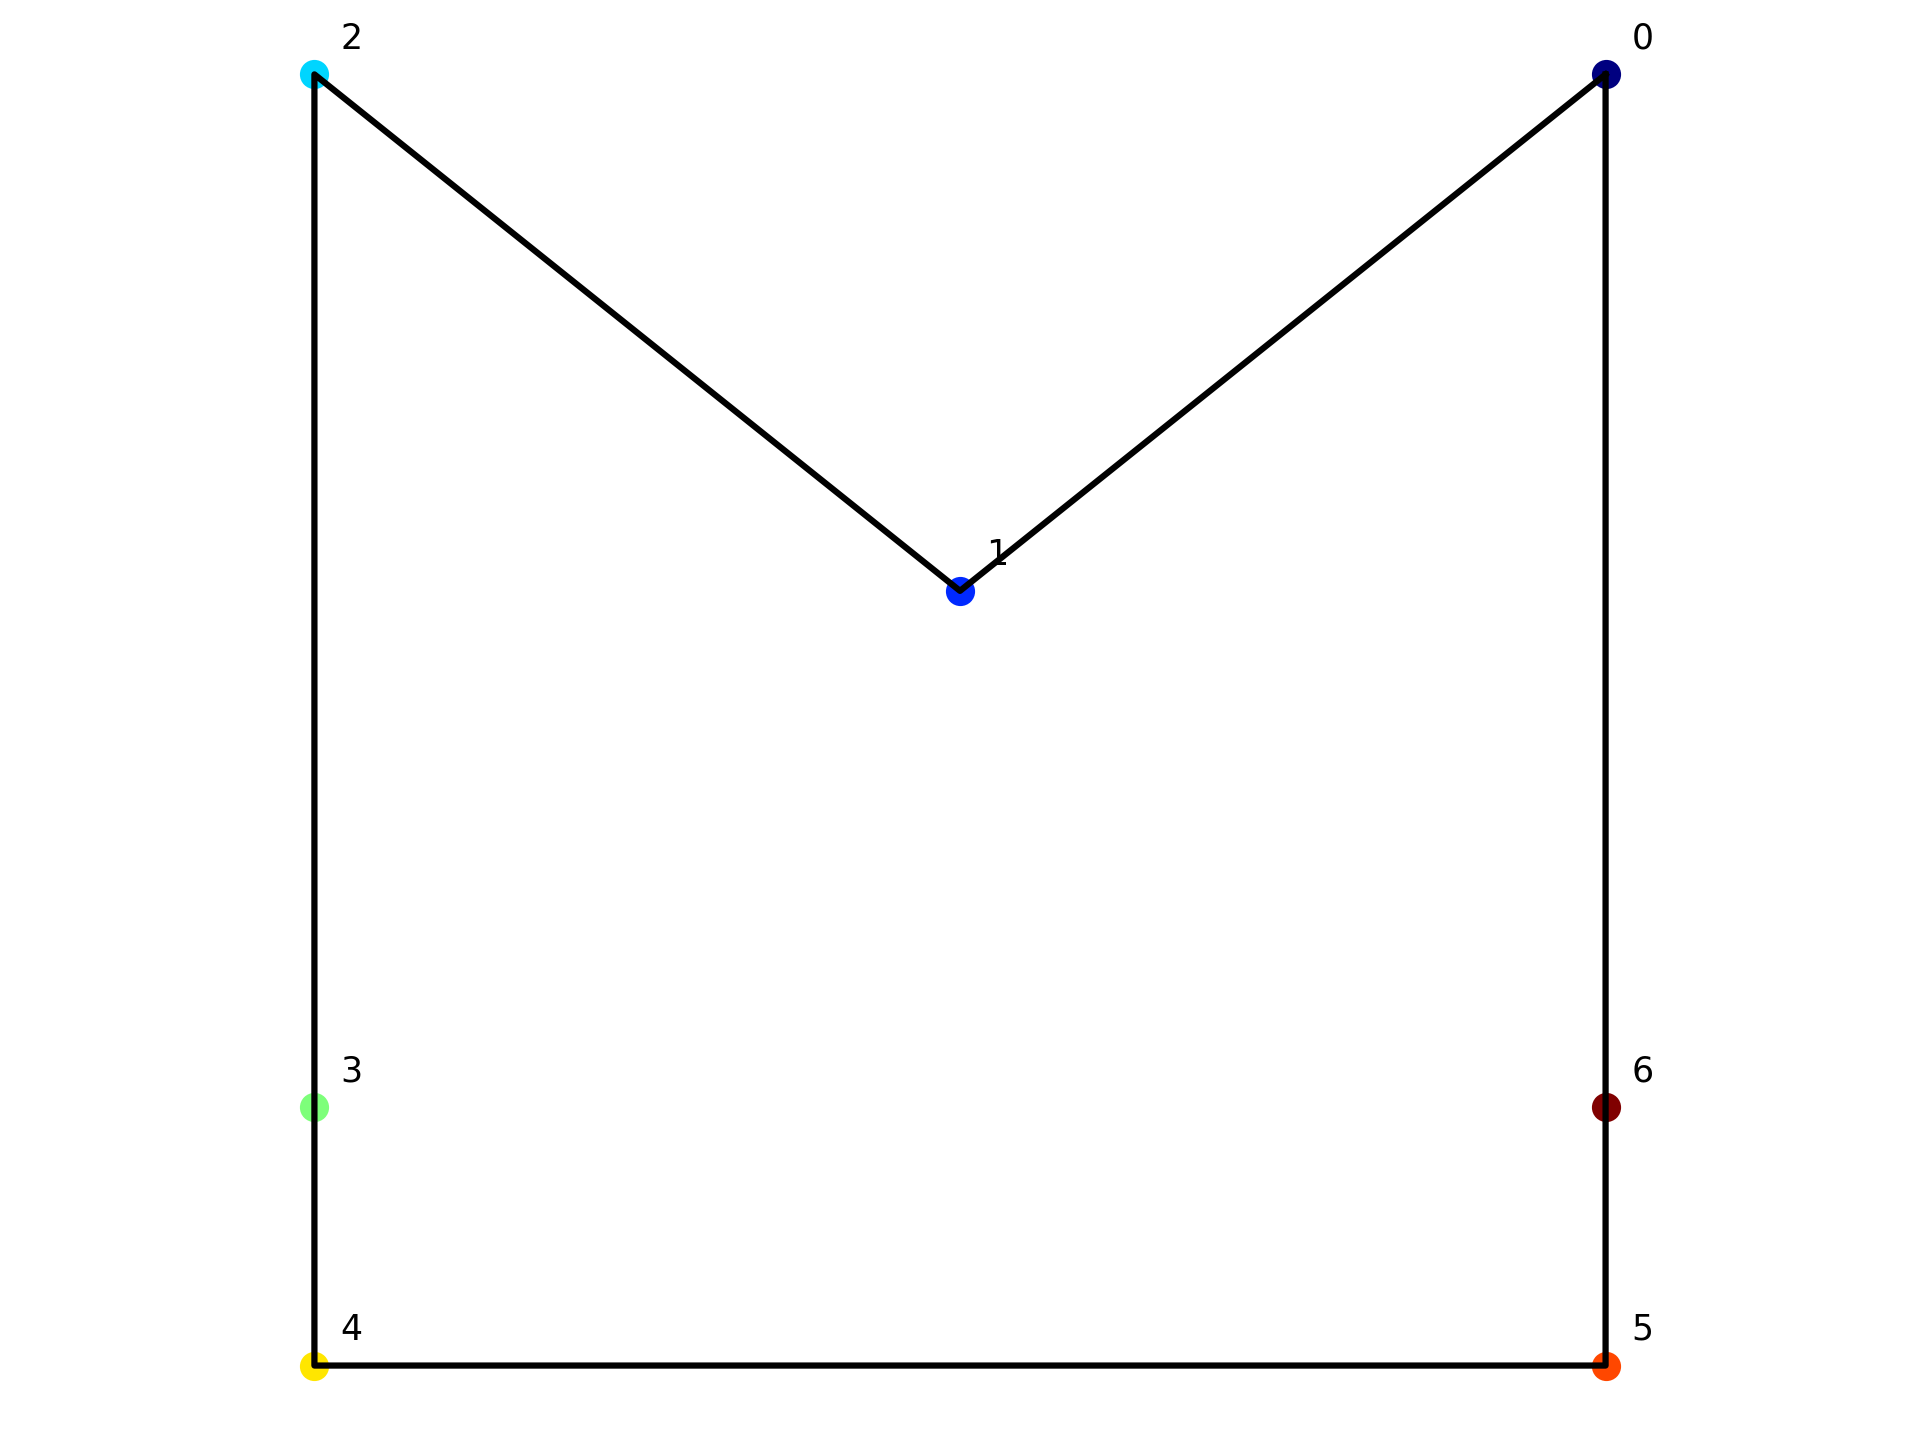
\includegraphics[width=\linewidth]{figures/poly3.png}
\end{subfigure}%
\begin{subfigure}{0.33\textwidth}
  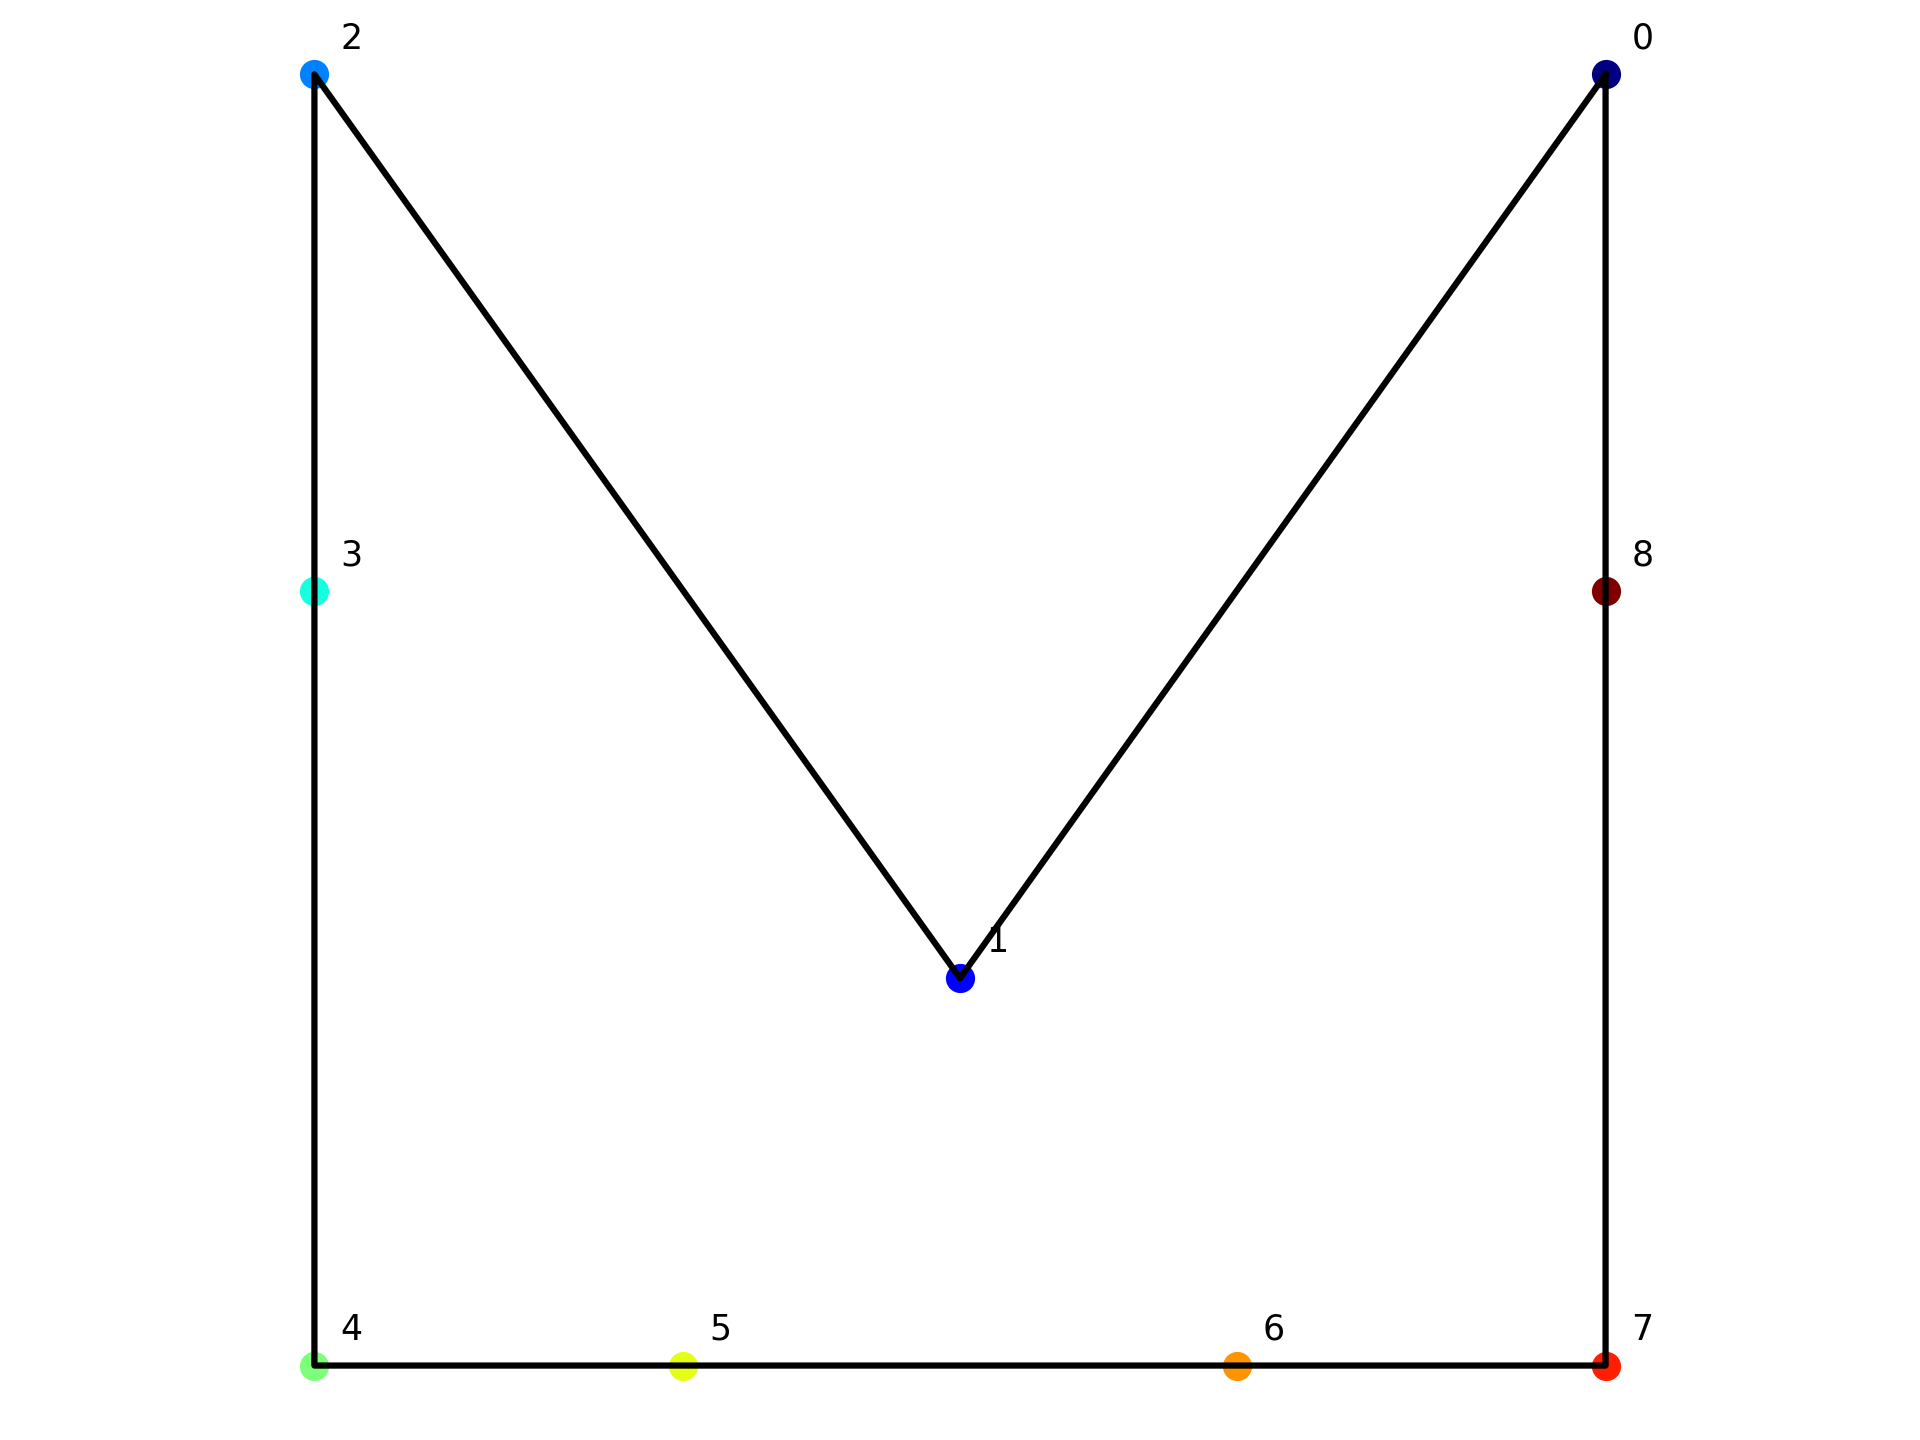
\includegraphics[width=\linewidth]{figures/poly2.png}
\end{subfigure}
\caption{Polygons with inserted "visibility event" vertices.}
\end{figure}


\begin{figure}
\centering
\begin{subfigure}{0.33\textwidth}
  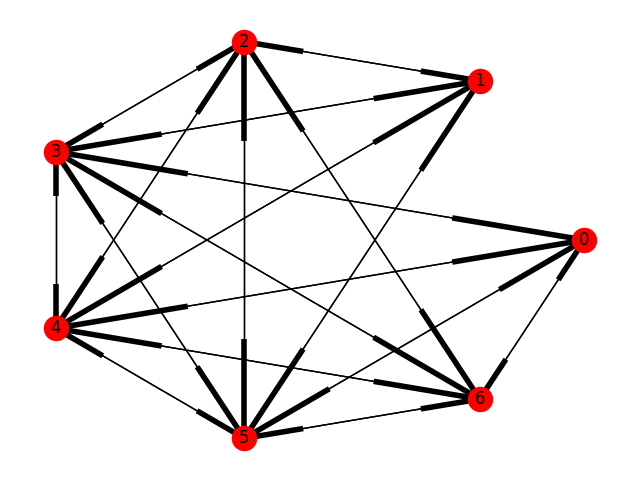
\includegraphics[width=\textwidth]{figures/graph1.png}
\end{subfigure}%
\begin{subfigure}{0.33\textwidth}
  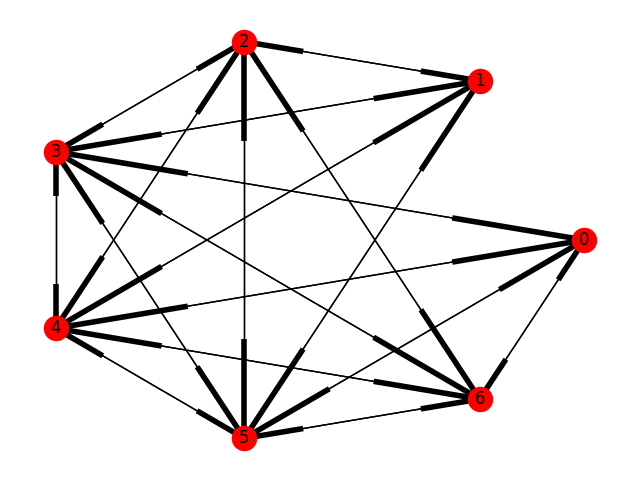
\includegraphics[width=\linewidth]{figures/graph3.png}
\end{subfigure}%
\begin{subfigure}{0.33\textwidth}
  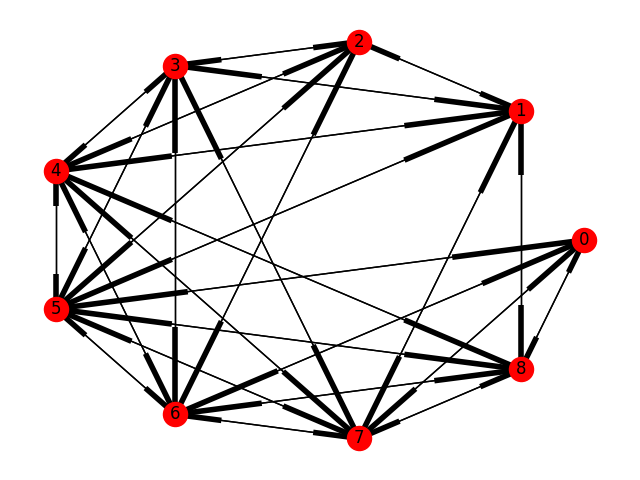
\includegraphics[width=\linewidth]{figures/graph2.png}
\end{subfigure}
\caption{Bounce visibility graphs (edge-to-edge visibility) for the polygons (edge between segments $i$
and $j$ implies that there exists a point and angle which allows transitions.}
\end{figure}


\begin{figure}
\centering
\begin{subfigure}{0.33\textwidth}
  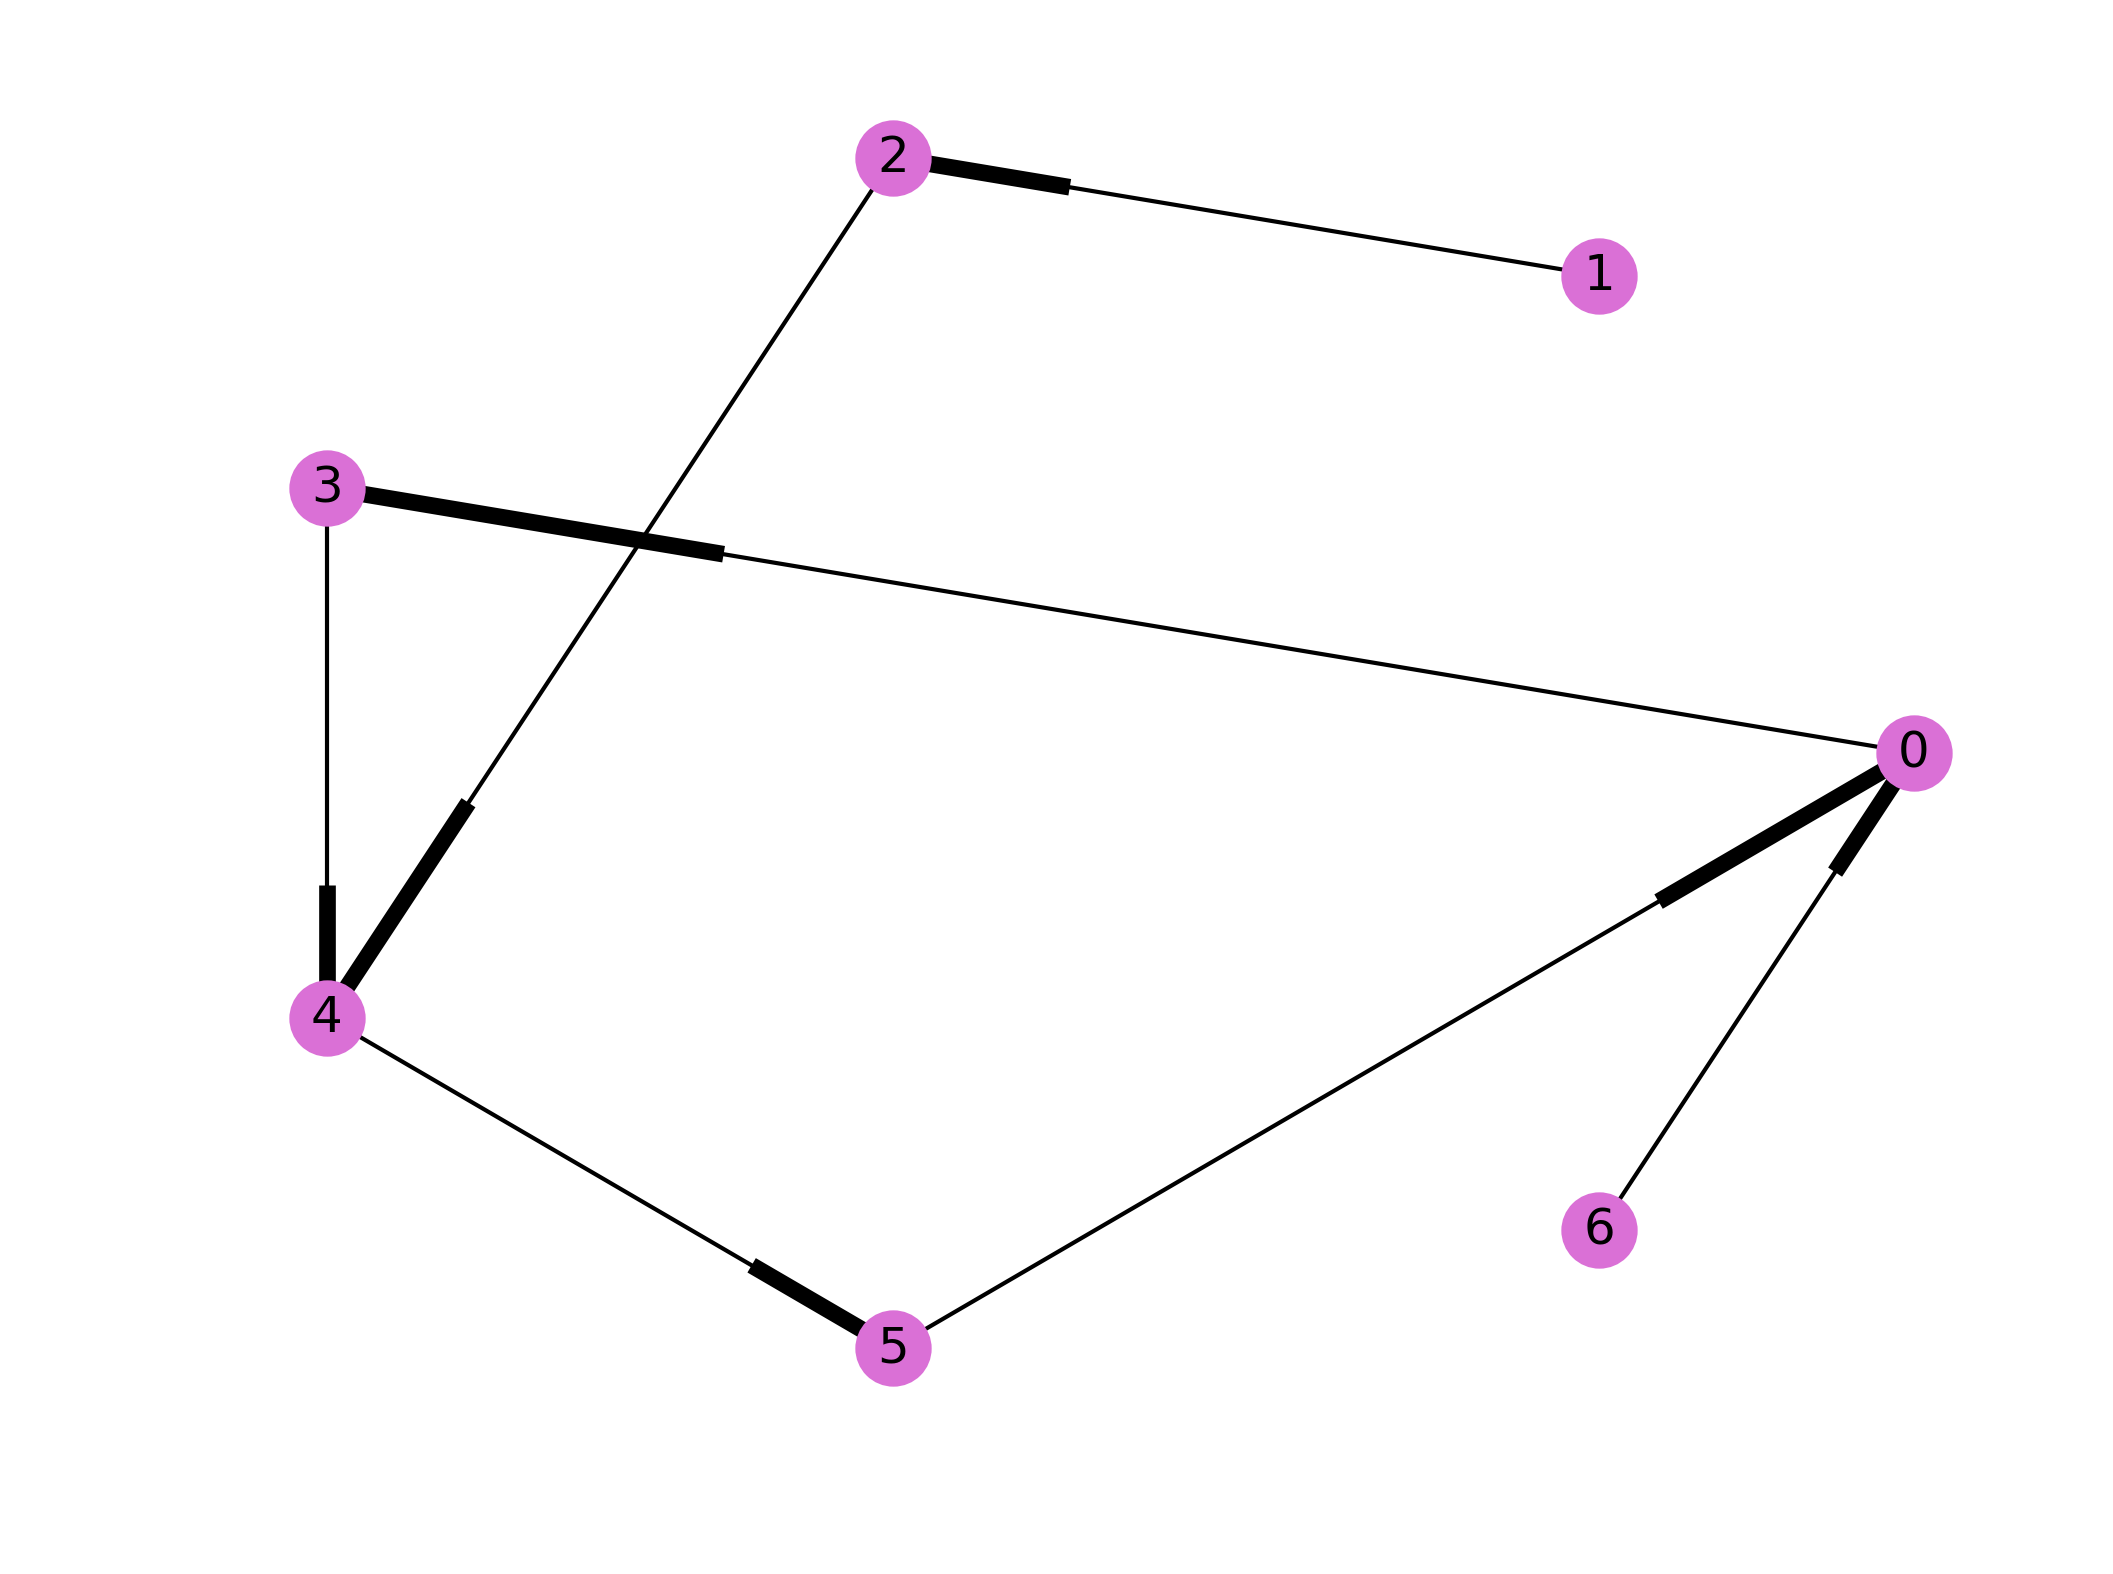
\includegraphics[width=\textwidth]{figures/reduced_graph1.png}
\end{subfigure}%
\begin{subfigure}{0.33\textwidth}
  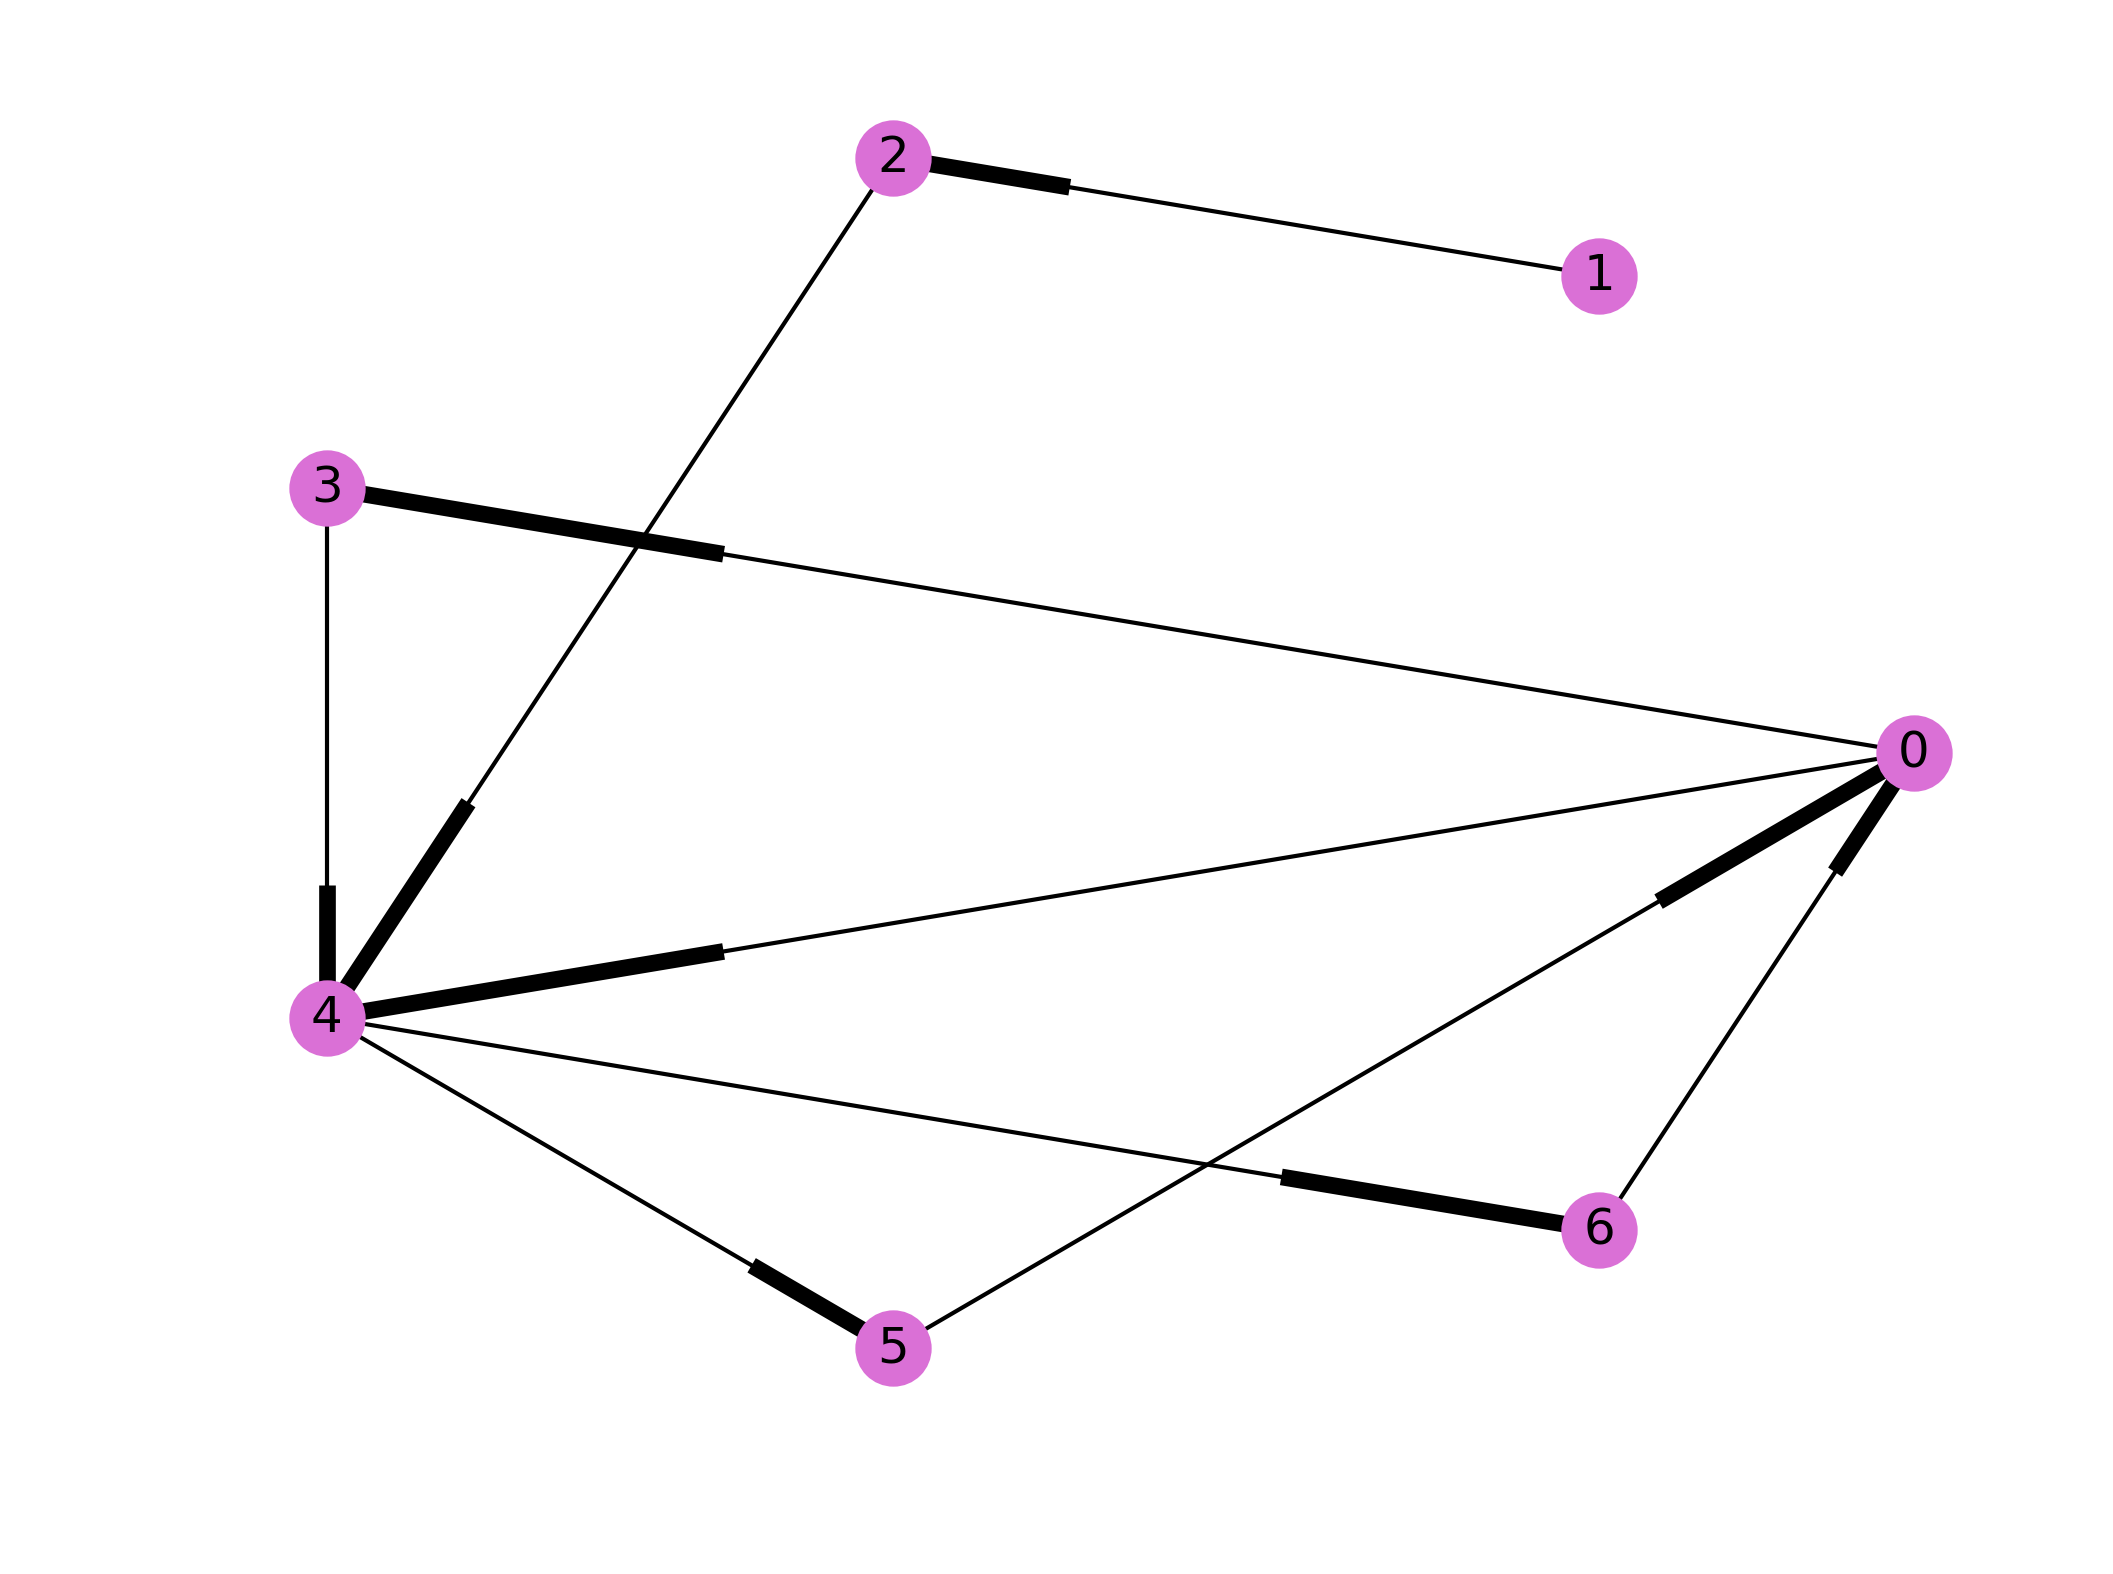
\includegraphics[width=\linewidth]{figures/reduced_graph3.png}
\end{subfigure}%
\begin{subfigure}{0.33\textwidth}
  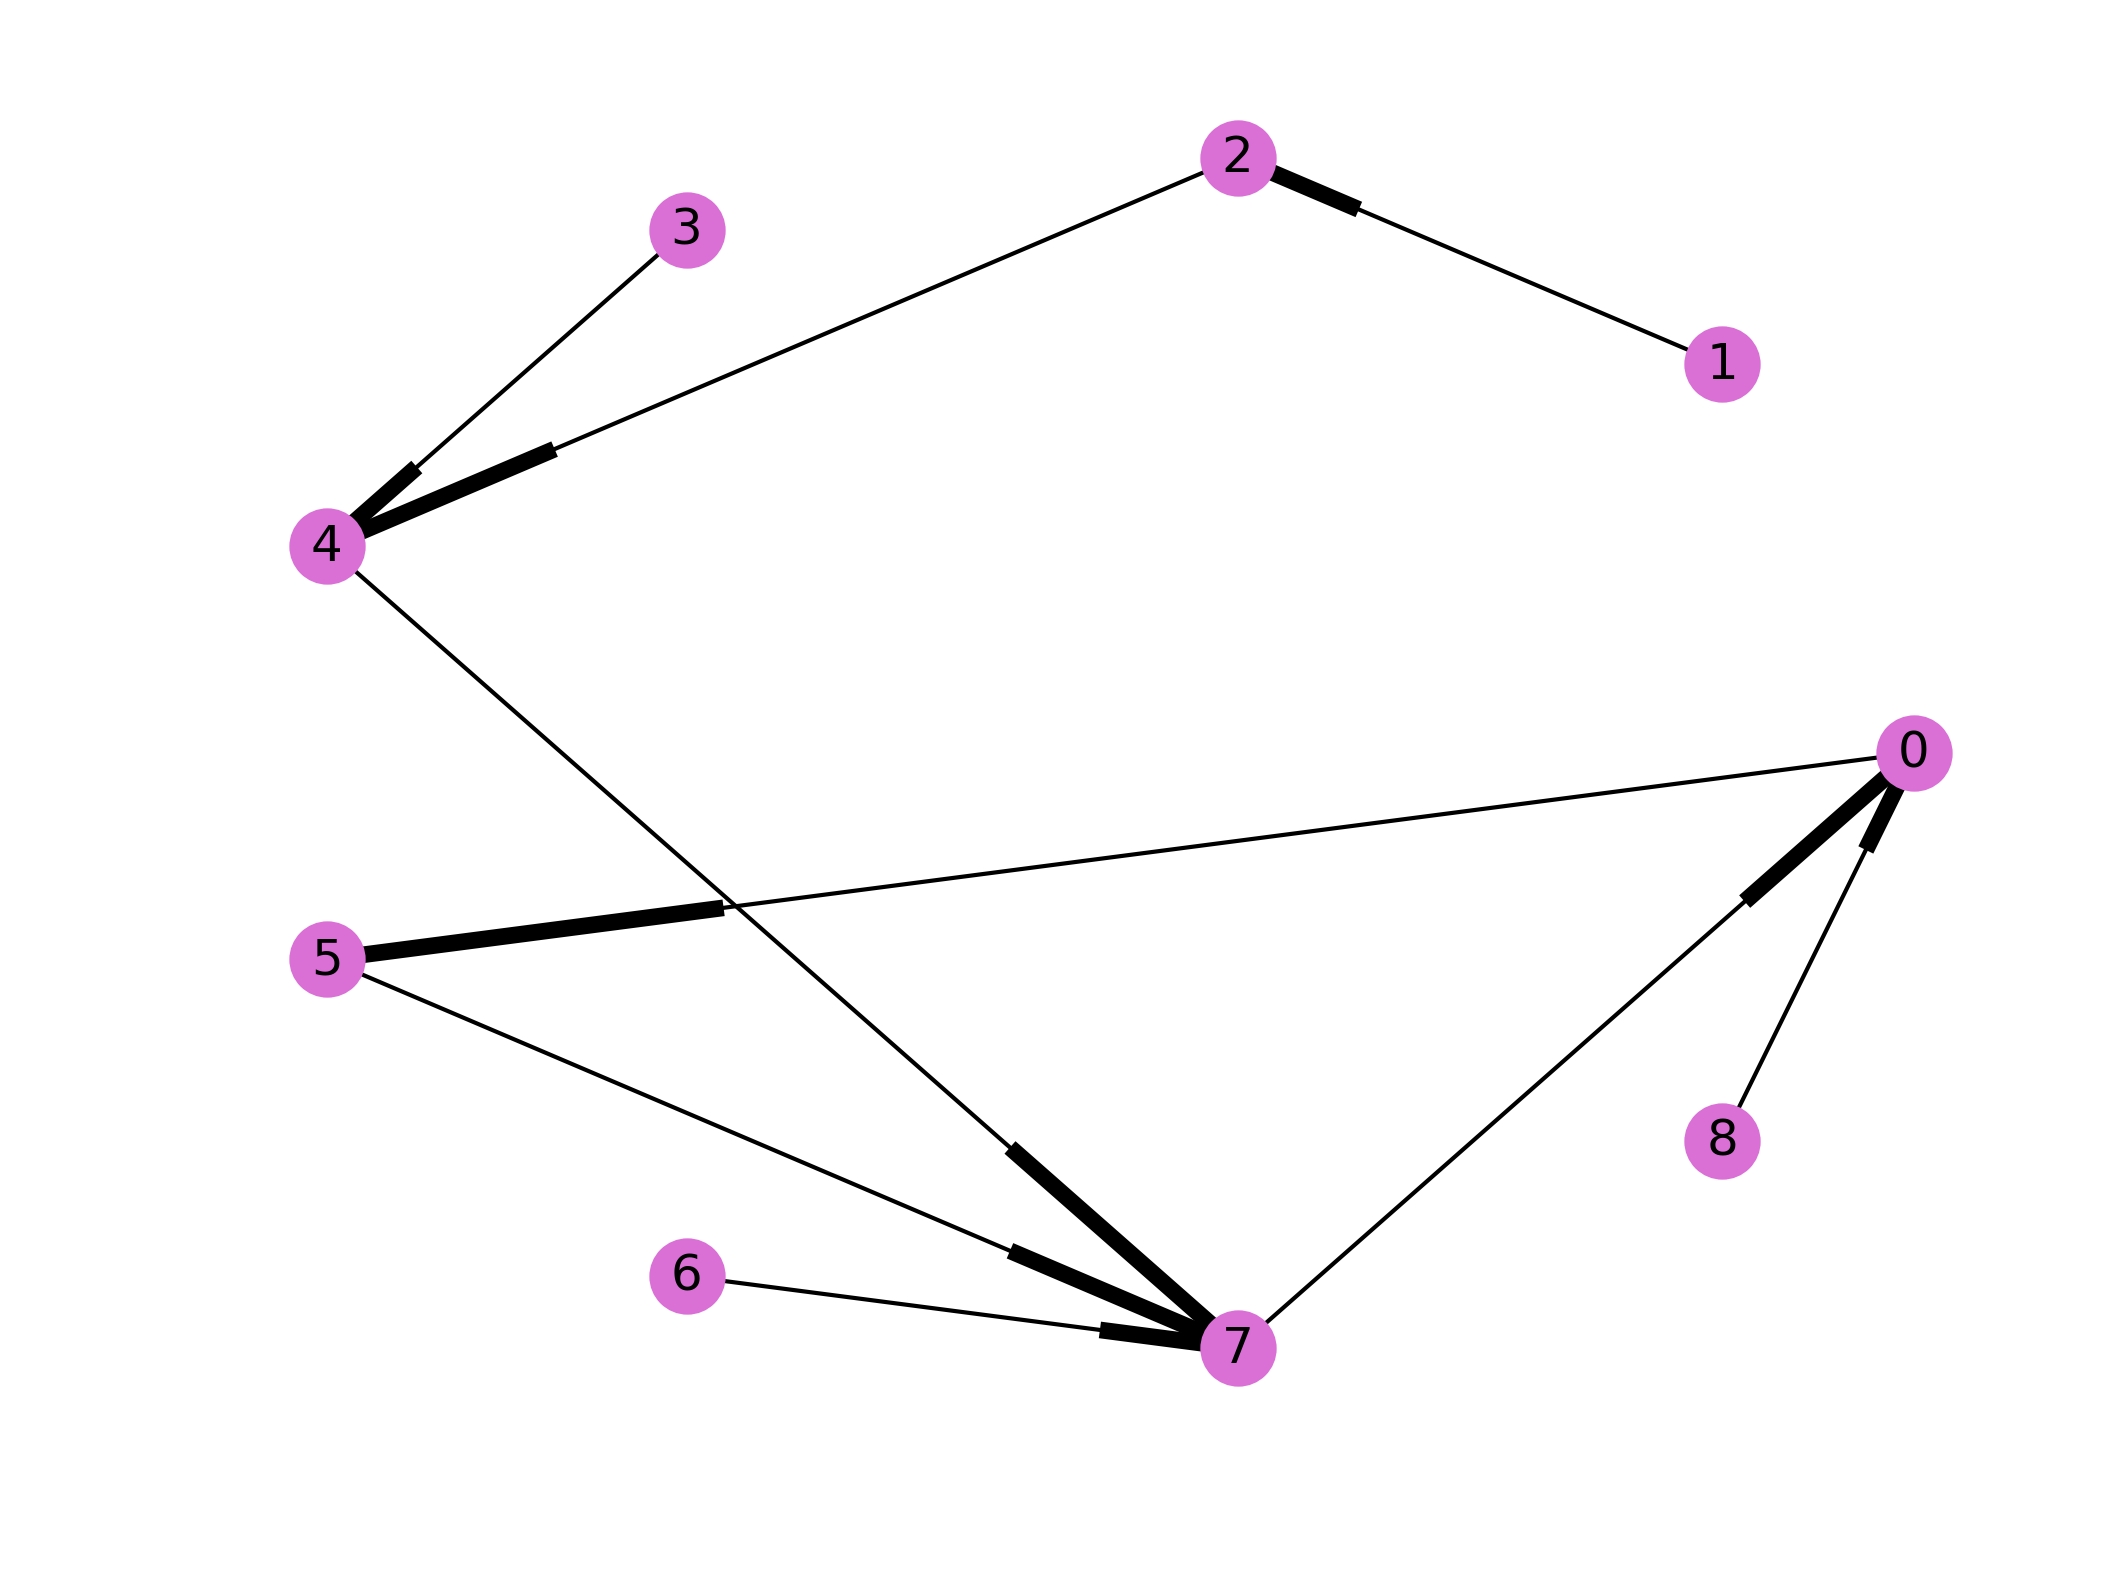
\includegraphics[width=\linewidth]{figures/reduced_graph2.png}
\end{subfigure}
\caption{Reduced bounce visibility graphs, for the angle range $0.15 < \theta <
0.19$ radians.}
\end{figure}


\begin{figure}
\centering
\begin{subfigure}{0.33\textwidth}
  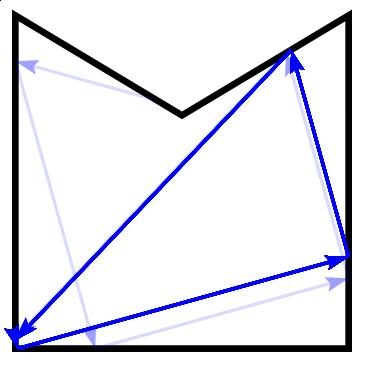
\includegraphics[width=\textwidth]{figures/poly1_limit_cycles.jpg}
\end{subfigure}%
\begin{subfigure}{0.33\textwidth}
  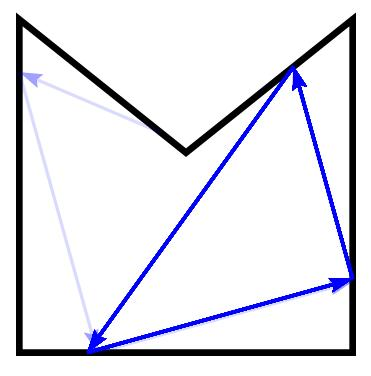
\includegraphics[width=\linewidth]{figures/poly3_limit_cycles.jpg}
\end{subfigure}%
\begin{subfigure}{0.33\textwidth}
  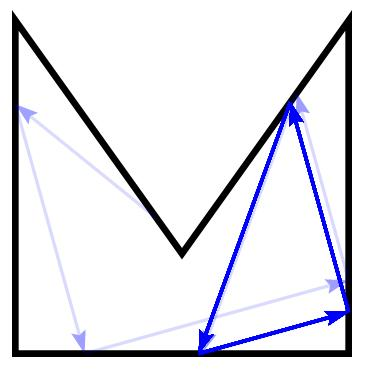
\includegraphics[width=\linewidth]{figures/poly2_limit_cycles.jpg}
\end{subfigure}
\caption{Limit cycles for $\theta = 0.17$ radians (counterclockwise from
boundary)}
\end{figure}


\end{document}
